\documentclass[titlestyle=hang,11pt]{elegantbook}

\author{~~~~~~陈~应~洪~~~~~~}
\email{985514056@qq.com}

\zhtitle{贝尔加教育}
\zhend{数学}
\entitle{BEI~ER~JIA~EDUCATION}
\enend{MATH}
\version{3.00}
\myquote{Victory won\rq t come to us unless we go to it.}
\logo{logo.png}
\cover{cover.pdf}
%%%%%%%%%%%


%%%%%%%%
%%%%%%%%%%%%%%%%%
%green color
   \definecolor{main1}{RGB}{0,120,2}
   \definecolor{second1}{RGB}{230,90,7}
   \definecolor{third1}{RGB}{0,160,152}
%cyan color
   \definecolor{main2}{RGB}{0,175,152}
   \definecolor{second2}{RGB}{239,126,30}
   \definecolor{third2}{RGB}{120,8,13}
%blue color
   \definecolor{main3}{RGB}{20,50,104}
   \definecolor{second3}{RGB}{180,50,131}
   \definecolor{third3}{RGB}{7,127,128}
\usepackage{draftwatermark} %水印包
\SetWatermarkText{贝尔加教育} %水印的标示
\SetWatermarkLightness{0.8} %水印的亮度
\SetWatermarkScale{0.7}     %水印的大小
\usetikzlibrary{snakes}
\usetikzlibrary{arrows.meta}
\usepackage{makecell}
\usepackage{lipsum}
\usepackage{texnames}
\usepackage{pgf,tikz,pgfplots}
\usepackage{tasks}%选择题宏包,tasks环境
\settasks{counter-format={tsk[A].},
	label-offset={0.4em},
	label-align=left,
	column-sep={2pt},
	item-indent={1pt},before-skip={-0.7em},after-skip={-0.7em}}
\usepackage{asymptote}

	
\begin{document}
\maketitle
\tableofcontents
\mainmatter

\chapter{解不等式}
\section{二次不等式与分式的解法}
\subsection{一元二次方程:$ax^2+bx+c=0(a \neq 0 )$}
\begin{enumerate}
	\item 解法 $x_1,x_2=\frac{-b\pm\sqrt{b^2-4ac}}{2a}$.
	\item 判别式  
	 \begin{enumerate}
		\item $\Delta >0$ ,有两个不相等的实数根.
		\item $\Delta =0$ ,有两个相等的实数根.
		\item $\Delta <0$ ,无实数根.
	\end{enumerate}
	\item 跟与系数的关系:$x_1+x_2=-\frac{b}{a}$、$x_1*x_2=\frac{c}{a}$.
	\item 根与函数的关系.
	\item 根与不等式的关系(等是不等的界).
\end{enumerate}
\subsection{二次函数:$y=ax^2+bx+c(a \neq 0 )$}

对称轴在内还是在外,在外为左还是右,内那边靠对称轴(max.min)。
\subsection{一元二次不等式}
\begin{enumerate}
	\item 一般式:$ax^2+bx+c>$或$ax^2+bx+c<0(a\neq 0)$
	\item 解法:函数法.
\end{enumerate}
\begin{figure}[h]
\includegraphics[scale=0.69]{1.png}
\end{figure}
\subsection{分式不等式}
\begin{enumerate}
	\item 一般式$\frac{f(x)}{g(x)}>0$或$\frac{f(x)}{g(x)}<0$.
	\item 解法:商化积$\frac{f(x)}{g(x)} >0$ $\Rightarrow f(x)g(x)>0$或$\frac{f(x)}{g(x)}<0$ $\Rightarrow f(x)g(x)<0$(穿根法).
\end{enumerate}
\section{例题分析}
\begin{example}解不等式 \par
(1).$2x^2-3x-2>0$   \hfil  (2)$-3x^2+6x>2$ \par
\vspace{2cm}
(3).$4x^2-4x+1>0$   \hfil  (4).$-x^2+2x-3>0$\\
\vspace{2cm}
\end{example}
\begin{example}解不等式\\
	(1).$(x-1)(x-a)<0$     \hfil   (2).$(x-1)(ax-1)>0$ \hfil  (3).$(x^2+6x+9)(x+1)>0$\\
	\vspace{2cm}
\end{example}
\begin{example}解不等式\\
	(1).$\dfrac{x-3}{x+7}<0$\hfil   (2).$\dfrac{1-2x}{x+4}\leq 0$ \hfil (3).$x^4-2x^2-8>0$\\
	\vspace{2cm}
\end{example}
\begin{example}解关于x的不等式$\frac{x-a}{x^2-3x-4}\leq(0\in R)$\\
	\vspace{2cm}
\end{example}
\begin{example}已知:方程$(m+1)x^2+2(2-m)x+2m+4=0(m\in R)$,求m为何值时一根大于3,一根小于3.\\
	\vspace{2cm}
\end{example}
\begin{example}解关于x的不等式\par
	(1)$x^2-2(a+1)x+1<0(a\in R)$\par
	\vspace{2cm}
	(2)$ax^2-(a-8)x+1>0(a\in R)$\par
	\vspace{2cm}
	(3)$kx^2-2(k-1)x+k+2>0(k\in R)$
	\vspace{2cm}
\end{example}
\chapter{绝对值不等式}
\section{含绝对值不等式的解法}
%%\subsection{含绝对值不等式的解法}
\begin{enumerate}
	\item 定义法:\begin{enumerate}
		\item $|x|<a(a>0)\Leftrightarrow -a<x<a$
		\item $|x|>a(a>0)\Leftrightarrow  x>a\text{或} x<-a$ 
		\item 含多个绝对值,用零点分区间.
	\end{enumerate}
	\item 公式法:\begin{enumerate}
		\item $|f(x)|<g(x)\Leftrightarrow -g(x)<f(x)<g(x)$
		\item $|f(x)|>g(x)\Leftrightarrow  f(x)>g(x)\text{或} f(x)<-g(x)$
	\end{enumerate}
\end{enumerate}
\section{例题分析}
\begin{example}解不等式\par
	(1).$|x-500|\leq 5$  \hfil   (2)$|2x+5|>7$\par
	\vspace{2cm}
	(3).$|x-a|<b$\hfil  (4).$|2x+1|+|x-2|>4$
	\vspace{2cm}
\end{example}
\begin{example}解不等式\par
	(1).$(1-|x|)(x+1)>0$  \hfil   (2)$|x^2-x-8|\geq x$\par
	\vspace{2cm}
	(3).$|\sqrt{x-2}-3|>1$\hfil  (4).$x^2-5|x|+6<0$\par
	\vspace{2cm}
	(5).$|x+7|-|3x-4|+\sqrt{3-2\sqrt{2}}>0$
	\vspace{2cm}
\end{example}
\begin{example}
	解关于x的不等式$(2x-1)a^2+(5x-2)a>3(x-1)(a\in R)$\\
	\vspace{2cm}
\end{example}
\begin{example}
   已知不等式$ax^2+bx+c>0$的解为$-3<x<1$,求不等式$cx^2+(a+b)x+6(b-a)<0$的解.
   \vspace{2cm}
\end{example}
\begin{example}解答\par
		(1).集合$\{x|0<|x-1|<3,x\in Z\}$的真子集个数.\par
		\vspace{2cm}
	(2).求使$\frac{\sqrt{3-|x|}}{\sqrt{|2x+1|-4}}$有意义的x的集合.\par
	\vspace{2cm}
	(3).已知$A=\{x||x-a|\leq 2\},B=\{x||x-1|\geq 3\}且A\cap B=\emptyset$则实数a的取值范围.\par
	\vspace{2cm}
	(4).若$a>0$,使不等式$|x-4|+|x-3|<a$的解集不是空集的a的范围.
	\vspace{2cm}
\end{example}
\begin{example}
	已知函数$f(x)=|x+1|-|x-2|$\par
	(1).求不等式$f(x)\geq 1$的解集;\par
	(2).若不等式$f(x)\geq x^2-x+m$的解集非空,求m的取值范围.\\
	\vspace{2cm}
	\end{example}
	\begin{example}
		已知$f(x)=|x+1|-|ax-1|$\par
		(1).当a=1时,求不等式$f(x)>1$的解集\par
		(2).当$x\in(0,1)$时不等式$f(x)>x$成立,求a的取值范围.
	\end{example}
	
\chapter{集合的表示与运算}
\section{集合的有关概念}
\begin{enumerate}
	\item 集合与元素.
	\item 元素的特征:确定性、互异性、无序性
	\item 集合的分类:\begin{enumerate}
		\item 有限集、无限集
		\item 空集、单元素集
		\item 可数集、不可数集
	\end{enumerate}
	\item 集合的表示:\begin{enumerate}
		\item 描述法:$ \{x|1<2<5\} $
		\item 例举法:\{1,2,3,4,5,6,7\}
		\item 韦恩图法
		\item 区间法  
	\end{enumerate}
	\item 子集与真子集
	\item 常用数集 ($\mathbb{Z}$ 、$\mathbb{R}$、$\mathbb{N}$、$\mathbb{N^*}$、$\mathbb{Q}$)
\end{enumerate}
\section{集合的运算}
\begin{enumerate}
	\item 交集
	\item 并集
	\item 补集
\end{enumerate}
\section{集合的运算律}
\section{例题}
\begin{example}
已知$A=\{x|2\leq x \leq 6\},B=\{x|2a\leq x\leq a+3\}$,若$B\subseteq A$,求实数a的取值范围.\\
\vspace{2cm}
\end{example}
\begin{example}
	在$\mathbb{R}$上定义运算$\oplus:x\oplus y=\frac{x}{2-y}$,关于x的不等式$x\oplus (x+1-a)>0$的解集是[-2,2]的子集,求实数a的取值范围.
\end{example}
\begin{example}
	$M=\{x\in \mathbb{R}|x^2+1=0.\}$ a=0,则下列关系式成立的是(\qquad)\par
	$A.a\in M$ \hfil $B.a\nsubseteq M$ \hfil  $C.\{a\}\supsetneqq M $ \hfil $D.\{a\}\subseteq M $
\end{example}
\begin{example}
$A=\{x|x=a^2+1,a\in N_+\}$;$B=\{x|x=b^2-4b+5,b\in N_+\}$,则下列关系式成立的是(\quad)\par
$A.A=B$  \hfil $B.A\subsetneqq B$ \hfil $C.A\supseteq B$ \hfil  $D.A\subseteq B$
\end{example}
\begin{example}
	$M=\{x,xy,\sqrt{x-y}\},N=\{0,|x|,y\}$若$M=N$,则$(x+y)+(x^2+y^2)+\cdots +(x^{100}+y^{100})=$(\qquad).\par
	$A.-200$  \hfil  $B.200$   \hfil  $C.-100$ \hfil  $D.0$
	
\end{example}
\begin{example}
$M=\{x|x=t^2,t\in Z\}$,$N=\{x\in R||x|<5\}$,则$M\cap N$的所有不同子集共有.(\quad)\par
$A.4$个\hfil  $B.7$个  \hfil    $C.8$个  \hfil    $D.10$个
\end{example}
\begin{example}
	$A=\{x|x=2n+1,n\in Z\}$,$B=\{x|x=4n\pm 1,n\in Z\}$,则下列关系式成立的是()\par
	$A.A=B$ \hfil $B.A\subseteq B$  \hfil  $C.A\supseteq B$ \hfil  $D.A\bigcap B=\emptyset $
\end{example}
\begin{example}
设$A\subset B$,则必为空集的是(\quad)\par
	$A.A\bigcap (\complement _U B)$ \hfil $B.B\bigcap (\complement _U A)$ \hfil  $C.(\complement _U A)\bigcap (\complement _U B)$ \hfil $D.A\bigcap B$
\end{example}
\begin{example}
	$A=\{x\in |mx+n \neq 0,m\neq 0\}$,$B=\{x\in R|px+q\neq 0\}$,则$\{x|(mx+n)(px+q)=0\}=$()\par
	$A.A\bigcap B$  \hfil   $B.A\bigcup B$ \hfil   $C.(\complement _R A)\bigcup (\complement _R B)$  \hfil   $D.(\complement _R A)\bigcap (\complement _R B)$
\end{example}
\begin{example}
	满足$\{1,3\}\bigcup B =\{1,3,5\}$的不同B的个数是(\quad).\par
	$A.1$  \hfil  $B.2$ \hfil   $C.3$ \hfil     $D.4$
\end{example}
\begin{example}	
	若$A\subseteq B \subseteq C$,集合A含3个元素,集合C含6个元素,则不同的集合B共有(\quad)\par
	$A.3$  \hfil  $B.4$ \hfil   $C.6$ \hfil     $D.8$
\end{example}
\begin{example}
	设全集$U=\{(x,y)|x,y\in R\},M=\{(x,y)|\frac{y-3}{x-2}=1\},N={(x,y|y\neq x+1)}$,则$\complement _U (M\bigcup N)=$(\quad).\par
	$A.\emptyset$  \hfil  $B.\{(2,3)\}$ \hfil   $C.(2,3)$ \hfil     $D.\complement _U N$
\end{example}
\begin{example}
	设$A=\{x\in R| x^2+px +q=0\},B=\{x\in R |x^2-px-2q=0\}$,若$A\bigcap B=\{-1\}$,求$A\bigcup B$.
\vspace{3cm}
\end{example}
\begin{example}
	设全集$U=\{1,2,4,a^2-a+1\},A=\{1,3a-2\},B={3,4}$,求$A\bigcap B$.
\vspace{3cm}
\end{example}
\begin{example}
	设$A=\{2,a^2-2a,6\},B={2,2a^2,3a-6}$,若$A\bigcap B=\{2,3\}$,求$A\bigcup B$.
\vspace{3cm}
\end{example}
\begin{example}
	设全集$U=\{x\in N_+ | x \leq 8 \}$,若$A\bigcap (\complement _U B)=\{1,8\}$,$(\complement _U A)\bigcap (\complement _U B)=\{4,7\}$,$(\complement _U A)\bigcap B=\{2,6\},$求集合A,B.
\vspace{3cm}
\end{example}
\begin{example}
	设$A=\{x|0<x<\leq 2\},B=\{x|ax^2-x+1=0\}$,若$\emptyset\subsetneqq B\subsetneqq R$,求证$A\bigcap B\neq \emptyset $
\vspace{3cm}
\end{example}
\begin{example}
	已知$A=\{1,3,x\},B=\{1,x^2\}$,若$B\bigcup (\complement _U B)=A$,求$\complement _U B$
	\vspace{3cm}
\end{example}
\begin{example}
	已知集合$A=\{x|x^2+px+q=0\},B=\{x|qx^2+px+1=0\},$若$A\bigcap B\neq \emptyset$且$A\bigcap (\complement _R B)=\{-2\}$,其中$p,q\neq 0$,求$p,q$的值.
\end{example}

\chapter{函数的概念}
\section{函数定义}
\begin{enumerate}
	
	\item  函数
	 \begin{enumerate}
		\item 	函数定义中的三性:任意性、存在性、唯一性.
		\item  函数的三要素:两域及对应法则.
	\end{enumerate} 
	\item 分段函数:对于定义内的不同取值范围内时,函数的解析式也不同.
	\item  复合函数

\end{enumerate}
\section{例题分析}
\begin{example}
	试判断一下各组函数是否表示同一函数?\par
	\begin{enumerate}
		\item $f(x)=\sqrt{x^2}$,\qquad $g(x)=\sqrt[3]{x^3}$
		\item $f(x)=\dfrac{|x|}{x}$,\qquad $g(x)=\begin{cases}
		1 & x \geq 0\\
		-1 & x<0
		\end{cases}$
		\item $f(x)=\sqrt[2n+1]{x^{2n+1}}$,\qquad $g(x)=(\sqrt[2n-1]{x})^{2n-1}(n\in N_+)$
		\item $f(x)=\sqrt{x}\sqrt{x+1}\qquad g(x) =\sqrt{x^2+x}$
		\item $f(x)=x^2-2x-1\qquad g(t)=t^2-2t-1$
	\end{enumerate}
\end{example}
\begin{example}
	设函数$f(x)=\begin{cases}
	 x-3 & (x\geq 100)\\
	f[f(x+5)]]  & (x<100)	
	\end{cases}
		$,求$f(89)$
\end{example}
\vspace{2.8cm}
\begin{example}
	函数$f(x)$对于任意实数x满足条件$f(x+2)=\frac{1}{f(x)}$,若$f(1)=-5$,则$f(f(5))$=
\end{example}
\vspace{2.5cm}
\begin{example}
已知函数$f(x)=\dfrac{\sqrt[3]{3x-1}}{ax^2+ax-3}$的定义域是$R$,则实数a的取值范围是(\quad)\par
$A.a>\frac{1}{3}$\hfil $B.-12<a\leq 0$  \hfil  $C.-12<a<0$  \hfil $D.a\leq \frac{1}{3}$
\end{example}
\begin{example} 求定义域:\par
	\begin{enumerate}
		\item 求函数$f(x)=\sqrt{x+1}+\dfrac{1}{2-x}$的定义域
		\vspace{2.5cm}
		\item 求函数$f(x)=\dfrac{\sqrt{x+3}}{\frac{1}{x}+2}$ 的定义域
		\vspace{2.5cm}
		\item 若函数$f(x)$的定义域为(0,3),则$f(x^2+2x)$的定义域是(\qquad)
		\vspace{2.5cm}
\item 	若函数$f(x+1)$的定义域为[-2,5],则$f(x)$的定义域是(\qquad)
\vspace{2.5cm}
\item 若函数$f(x+1)$的定义域为[-2,5],则$f(\frac{1}{x}+1)$的定义域是(\qquad)
	\end{enumerate}
	\vspace{2.3cm}
\end{example}
\begin{example} 求下列值域:\par
	$y=\dfrac{3x+1}{x-2}$\hfil $y=|x-1|+|x+4|$\hfil $y=|2x-1|+|x+4|$ \par
	\vspace{2.3cm}
	$y=-x^2-2x+3(-5\leq x \leq -2)$ \hfil $y=\dfrac{3x^2+3x+1}{x^2+x-1}$ \hfil $y=x+\sqrt{2x-1}$
	\par
	\vspace{2.3cm}
		$y=\dfrac{x^2}{x^2+1}$\hfil $y=\sqrt{5+4x-x^2}$
		\vspace{2.5cm}
\end{example}
\newpage
\begin{example} 求解析式
	\begin{enumerate}
	\item  已知$f(x+\dfrac{1}{x})=x^3+\dfrac{1}{x^3}$,求$f(x)$
	\vspace{2.5cm}
	\item 已知$f(\dfrac{2}{x}+1)=x^2$,求$f(x)$
	\vspace{2.5cm}
	\item 已知$f(\sqrt{x}+1)=x+2\sqrt{x}$,求$f(x)$
	\vspace{2.5cm}
	\item 已知$f(x)$是一次函数,且满足$3(x+1)-2f(x-1)=2x+17$,求$f(x)$
	\vspace{2.5cm}
	\item 已知$f(x)$满足$2f(x)-f(\dfrac{1}{x})=3x$,求$f(x)$
		\end{enumerate}
\end{example}

\chapter{函数的单调性}
\section{例题分析}
\begin{example}
	用定义证明函数的单调性:\par
	(1).证明函数$f(x)=ax+b$的单调性。\par
\vspace{2.8cm}
	(2).证明函数$f(x)=x^3$的单调性。\par
	\vspace{2.8cm}
	(3).证明函数$f(x)=x+\sqrt{x^2+1}$的单调性。\par
	\vspace{2.8cm}

\end{example}
\begin{example}
已知函数分$f(x)=\dfrac{a+bx}{a-bx},x\in [-1,1]$	\par
(1).$a=1,b=3$时,证明$f(x)$在[-1,0]上是增函数.\par
(2).a>b>0,时,证明$f(x)$在[-1,1]上是增函数.\par
(3).求函数f(x)的值域。\par
\vspace{5.5cm}
\end{example}
\begin{example}\par
	(1).证明函数$f(x)=\dfrac{x}{x^2+1}$在(-1,1)上是增函数.\par
	(2).证明函数$f(x)=\dfrac{kx}{x^2+1}$在(-1,1)上是增函数.\par
	(3).证明函数$f(x)=ax+\dfrac{b}{x}(a>0,b>0,x\in(0,+\infty))$的单调性\par
	\vspace{4cm}
\end{example}
\begin{example}
	已知函数$f(x)=x^2-2ax+a^2-1$\par
	(1).若函数$f(x)$的区间[0,2]上是单调的,求实数a的取值范围;\par
	(2).当$x\in [-1,1]$时,求函数$f(x)$的最小值g(t),并画出g(t)的函数图像。
	\vspace{4cm}
\end{example}
\begin{example}
	求函数$f(x)=3x^2-x+2(x\in [m,n])$的值域.
\end{example}
\chapter{函数的奇偶性}
\section{例题分析}
\begin{example}
	已知偶函数$f(x)$在区间[0,4]上是增函数,试比较$f(-3)$与$f(\pi)$的大小.
\end{example}
\vspace{2.5cm}
\begin{example}
	若奇函数$f(x)$在[3,7]上的最小值是5,那么$f(x)$在[-7,-3]上(\qquad)\par
	A.最小值是5\hfil B.最小值是-5  \hfil  C.最大值是-5   \hfil  D.最大值是5
\end{example}
\begin{example}
$f(x)$是定义在$R$上的奇函数,又$f(x)$在区间(0,+$\infty$)上是增函数,且$f(1)=0$,则满足$f(x)>0$的x的取值范围集合是(\qquad)
\end{example}
\vspace{2.5cm}
\begin{example}
设$f(x)$是定义在$R$上的奇函数,又$f(x+2)=-f(x)$,当$0\leq x \leq 1$时,$f(x)=x$,则$f(7.5)$等于(\qquad) 
\end{example}
\vspace{2.5cm}
\begin{example}
如果函数$f(x)$在$R$上为奇函数,在[-1,0)上是增函数,且$f(x+2)=-f(x)$,试比较$f(\frac{1}{3}),f(8.5),f(1)$的大小关系(\qquad)
\end{example}
\vspace{2.5cm}
\begin{example}
若$f(x)$为奇函数,且在(0,+$\infty$)内是增函数,又$f(-3)=0$,则$xf(x)<0$的解集为(\qquad)
\end{example}
\vspace{2.5cm}
\begin{example}
设函数$y=f(x)$对于任意的$x,y\in R$都有$f(x+y)=f(x)+f(y)$,且f(x)不恒为零,判断f(x)的奇偶性.
\end{example}
\vspace{2.5cm}
\begin{example}
f(x)是定义在$R$上的偶函数,且当$x\leq 0$时,$f(x)=x^2-x$,求$f(x)$的解析式.并画出函数图象,求出函数的值域。
\end{example}
\vspace{2.5cm}
\begin{example}
已知$f(x)$是定义在$R$上的奇函数,当$x>0$时$f(x)=x^2-4x+3$,求$f(x)$的解析式.
\end{example}
\vspace{2.5cm}
\begin{example}
已知函数$f(x)$是定义在区间[-2,2]上的偶函数,当$x\in [0,2]$时,f(x)是减函数,如果不等式$f(1-m)<f(m)$成立,求实数m的取值范围
\end{example}
\vspace{2.5cm}
\begin{example}
	已知函数f(x)定义域$R$,为对任意的$x_1,x_2\in R$都有$f(x_1+x_2)=f(x_1)+f(x_2)$且$x>0$时$f(x<0)$,f(1)=-2,试判断在区间[-3,3]上$f(x)$是否有最大值和最小值?如果有试求出最大值和最小值,如果没有请说明理由. 
\end{example}
\vspace{2.5cm}
\begin{example}
已知函数$f(x)$定义域$R$,为对任意的$x_1,x_2\in R$都有$f(x_1+x_2)=f(x_1)f(x_2)$且$x>0$时,$0<f(x)<1$,求$f(0)$的值并求$x<0$时$f(x)$的取值范围.
\end{example}
\vspace{2.5cm}
\begin{example}
已知$f(x)$是定义在$R$上的奇函数,当$x\geq$时,$f(x)=x^2-2x$,则f(x)在R上的表达式是\par
$A.f(x)=x^2-2x$\hfil $B.f(x)=x(|x|-1)$\par
$C.f(x)=|x|(x-2)$\hfil $D.f(x)=x(|x|-2)$
\end{example}
\begin{example}
函数$f(x)$是定义在[-6,6]上的偶函数,且在[-6,0]上是减函数,则(\qquad)\par
$A.f(x)+f(4)>0$\hfil $B.f(-3)-f(2)<0$\par
$C.f(-2)+f(-5)<0$\hfil $D.f(4)-f(-1)>0$
\end{example}
\begin{example}
设$f(x)$是定义在$R$上的任意一个增函数,令$F(x)=f(x)-f(-x)$,则$F(x)$必是(\qquad)\par
A.增函数且是奇函数      \hfil    B.增函数且是偶函数 \par
 C.减函数且是奇函数       \hfil   D.减函数且是偶函数
\end{example}
\begin{example}
	设$f(x),g(x)$都是奇函数,$F(x)=f(x)+g(x)+3$,若$F(5)=9$,$F(-5)$=(\qquad)\par
	$A.3$  \hfil $B.-3$  \hfil $C.-6$  \hfil $D.-9$ 
\end{example}
\begin{example}
设$f(x),g(x)$都是奇函数,且$F(x)=af(x)+bg(x)+2$,若在$(0,+\infty)$上$F(x)$有最大值8,则在$(\infty,0)$上$F(x)$有(\qquad)\par
A.最小值-8  \hfil       B.最大值-8  \hfil     C.最小值-4  \hfil         D.最小值-6
\end{example}
\begin{example}
函数$f(x)=\dfrac{\sqrt{1-x^2}}{|x+3|-3}$是(\qquad)\par
A. 奇函数  \hfil  B. 偶函数 \hfil   C. 既奇又偶函数  \hfil D. 没有确定的奇偶性
\end{example}
\begin{example}
若$f(x)=ax^2+bx+c(a\neq 0)$是偶函数,则$g(x)=ax^3+bx^2+cx$是(\qquad)\par
A. 奇函数 \hfil B. 偶函数 \hfil  C. 既奇又偶函数 \hfil   D. 没有确定的奇偶性
\end{example}
\begin{example}
下列命题:(1)偶函数图象一定与y轴相交(2)奇函数图象一定过原点(3)偶函数图象关于y轴对称(4)既奇又偶函数一定满足$f(x)=0$,其中真命题个数是(\qquad)\par
A. 1    \hfil   B. 2   \hfil    C. 3   \hfil     D. 4
\end{example}
\begin{example}
若奇函数$f(x)$在区间[3,7]上是增函数,且最小值为5,那么在区间[-7,-3]上是\par
A.增函数且最小值为-5 \hfil   B.增函数且最大值为-5  \par
C.减函数且最小值为-5  \hfil  D.减函数且最大值为-5
\end{example}
\begin{example}
下列四个命题:\par
(1)$f(x)=1$是偶函数;\par
(2)$g(x)=x^3,x\in (-1,1]$是奇函数;\par
(3)若$f(x)$是奇函数,$g(x)$是偶函数,则$H(x)=f(x)g(x)$一定是奇函数;\par
(4)函数$y=f(|x|)$的图象关于y轴对称。其中正确的命题个数是(\qquad)\par
A.1    \hfil       B.2   \hfil
        C.3    \hfil           D.4
\end{example}
\begin{example}
已知$f(x)=x^4+ax^3+bx-8$,且$f(-2)=10$,则$f(2)$=\underline{\qquad}
\end{example}
\begin{example}
判断下列函数的奇偶性:\par
(1).$ f(x)=\begin{cases}
 x+1(x>0)\\
1(x=0)\\
-x+1(x<0) \end{cases} $ \underline{\qquad} \par
(3).$f(x)$不恒为0,且对$a,b\in R $恒有$f(a+b)=f(a)+f(b)$\underline{\qquad}

\end{example}
\begin{example}
	已知$f(x)$是定义在$R$上的奇函数当x>0时,$f(x)=\sqrt{x}+1$,则$f(2)$=\underline{\qquad}
\end{example}
\begin{example}
是否存在常数$m,n$,使函数$f(x)=(m^2-1)x^2+(m-1)x+n+2$为奇函数?
\end{example}
\vspace{2.5cm}
\begin{example}
已知函数$f(x)$满足$f(x+y)+f(x-y)=2f(x)f(y)(x,y\in R)$试证明f(x)是偶函数。
\end{example}
\vspace{2.5cm}
\begin{example}
已知函数$y=f(x)$为奇函数,在$(0,+\infty)$内是减函数,且$f(x)<0$,试问:$F(x)=\dfrac{1}{f(x)}$在$(-\infty,0)$内增减性如何?并证明.
\end{example}
\chapter{指数函数与对数函数}
\section{指数运算与对数运算}
\begin{enumerate}
	\item 指数的性质
	\begin{enumerate}
		\item $a^n=a·a·a......(a\in R)$
		\item $a^{-n}=\frac{1}{a^n} (a\neq 0)$
		\item  $a^0=1 (a\neq 0)$
		 \item $a^{\frac{m}{n}}=\sqrt[n]{m}$
	\end{enumerate}
\item  指数的运算
  \begin{enumerate}
  	\item $(a^m)^n=a^{(m·n)}$
  	\item $a^m·a^n=a^{(m+n)}$
  	\item $(a·b)^n=a^n·a^b$
  \end{enumerate}
\item 对数的性质
     \begin{enumerate}
     	\item $a^b \Longleftrightarrow b=\log_aN (a>0,a\neq 0)$
     	\item $a^0=1\Longrightarrow \log_a1=0$
     	\item  $a^1=a \Longrightarrow \log_a a$ 
     	\item $a^{\log_a x}=x$
     	\item $\log_a a^x=x$
     	\item $log_ab=\dfrac{\log_c b}{\log_c a} \Longrightarrow (\log_a b=\dfrac{1}{\log_b a};\log_a b=\log_{a^N}b^n)$
     	\item  $\log_{a^N}b=\frac{1}{n}\log_ab$
     \end{enumerate}
 \item 对数的运算
 \begin{enumerate}
 	\item $\log_a(M·N)=\log_a M +\log_a N$
 	\item $\log_a(\frac{M}{N})=\log_a M-\log_aN$
 	\item $\log_aM^n=nlog_a M$
 \end{enumerate}
 
\end{enumerate}
\section{例题分析}
\begin{example} 比较下来各数的大小.\\
	(1)$0.3^2\hspace{0.5cm} \log_2\frac{1}{3}\hspace{0.5cm}\log_3\frac{1}{9} \hspace{0.5cm} \log_{\frac{1}{2}}5\hspace{0.5cm} \log_4 15 \hspace{0.5cm} \log_{\frac{1}{2}}{\frac{1}{15}}	$~\vspace*{0.6cm}\\
	(2)$\log_{0.5}0.6 \hspace{0.5cm} \log_{\sqrt{2}}0.5 \hspace{0.5cm} \log_{\sqrt{3}}\sqrt{5}$\\
\end{example}

\begin{example}求下列函数的单调性、最值\par
	$(1)y=3^{|x|}-1$  \hfil $y=2^{x^2-x+1}$\par
	\vspace*{3cm}
	$(3)y=4^x-x^{x+1}+1$\hfil $(4)y=\log_a(x^2-1)$\par
	\vspace*{3.5cm}
	$(5)y=\log_2(x^2-3x+2)$\hfil $(6)y=(\log_2x)^2-3\log_2x+2,x\in[1,2]$
	\vspace*{3.5cm}
\end{example}
\begin{example}判断下列函数的奇偶性\par
$(1)f(x)=\dfrac{1}{2^x-1}+\dfrac{1}{2}$\par
\vspace{3cm}
$(2)f(x)=\lg\dfrac{1-x}{1+x}$\par
\vspace{3cm}
$(3)f(x)=\ln(\sqrt{1+x^2}-x)$\par
\vspace{3cm}
\end{example}
\begin{example}已知函数$f(x)=\lg(ax^2+2x+1)$\par
	(1)若$f(x)$的定义域为$R$,求实数a的取值范围.\par
	\vspace{4cm}
	(2)若$f(x)$的值域为$R$,求实数$a$的取值范围.\par
	\vspace{4cm}
\end{example}
\begin{example}分别求函数$f(x)=2^x+2^{-x}$和$g(x)=\dfrac{1-2^x}{4^x}$的定义域、值域\par

\end{example}
% Table generated by Excel2LaTeX from sheet 'Sheet1'
\begin{table}
	\centering
	\caption{TableName}
	\begin{tabular}{|l|l|l|l|}
		\hline
		
		Id & Name & Age & Gender\\ \hline
		1 & Lawrence & 39 & M\\ \hline
		2 & Oliver & 25 & M\\ \hline
		3 & Roberta & 17 & F\\ \hline
		4 & Bamboo & 70 & F\\ \hline
		
	\end{tabular}
\end{table}


\chapter{概率的初步}
\section{随机事件的概率}
\subsection{事件的定义}
\begin{theorem}{事件的定义}{31}
	\begin{enumerate}[noitemsep]
	\item 必然事件:在一定条件下,有些事必然会发生,这样的事件叫做必然事件.
	\item 不可能事件:在一点条件下,有些事件必然不会发生,这样的事件叫做不可能事件.
	\item 随机事件:在一定条件下,可能发生也可能不发生的事件叫做随机事件.
	\end{enumerate}
\end{theorem}
\subsection{事件的分类}
$$
\text{事件} \begin{cases}  
\text{确定性事件} \smash[t]{\begin{cases}
	\text{必然事件} \\  \text{不可能事件}
	\end{cases}}
\\
\text{随机事件}
\end{cases}
$$
\subsection{概率}
\begin{theorem}{概率}{31}
	\textbf{概率的定义:} 一般的,对于一个随机事件A,我们把刻画其发生可能性的大小的数值,称为随机事件A发生的概率,记为P(A)
\end{theorem}
\chapter{点、直线、平面之间的位置关系}
\section{空间点、直线、平面之间的位置关系}
\subsection{平面}
\begin{theorem}{公理}{31}
	\begin{enumerate}[noitemsep]
	\item 如果一条直线上的两点在一个平面内,那么这条直线在此平面内.\\
	$A\in l,B\in l,且A\in \alpha ,B\in \alpha  \Rightarrow l\subset \alpha $
	\item 过不在一条直线上的三个点,有且只有一个平面
	\item 如果两个不重合的平面有一个公共点,那么他们有且只有一条过该点的公共直线.\\
	$P\in \alpha ,且 P\in \beta \Rightarrow \alpha \cap \beta =l ,且 P\in l  $
\end{enumerate}
\end{theorem}
\subsection{空间中直线与直线之间的位置关系}

\begin{theorem}{公理}{31}
\begin{enumerate}[noitemsep]
	\item  平行于同一条直线的两条直线相互平行(平行线的传递性).
	\item 空间中如果两个角的两边分别对应平行,那么这两个角相等或者互补.
\end{enumerate}
\end{theorem}
\subsection{空间中直线与平面之间的位置关系}
\begin{enumerate}
\item	直线在平面内$\textemdash$ 有无数个公共点.
\item     直线与平面相交$\textemdash $ 有且只有一个公共点.
\item    直线与平面平行$\textemdash $  无公共点.
\end{enumerate}
\subsection{平面与平面之间的位置关系}
\begin{enumerate}
	\item 两个平面平行$\textemdash $没有公共点.
	\item 两个平面相交$\textemdash $有一条直线.
\end{enumerate}
\section{直线、平面平行的判定及其性质}
\subsection{直线与平面平行的判定}
\begin{theorem}{}{}
	平面外一条直线与此平面内的一条直线平行,这该条直线与此平面平行(线线平行$\Rightarrow$)线面平行.
\end{theorem}
\subsection{平面与平面平行的判定}
\begin{theorem}{}{}
	一个平面的内的两条相交直线与另一个平面平行,则这两个平面相互平行(线面平行$\rightarrow$面面平行)。
\end{theorem}
\subsection{直线与平面平行的性质}
\begin{theorem}{}{}
	一条直线与一个平面平行,则过这条直线的任意平面与该平面的交线与该直线平行.
\end{theorem}
\subsection{平面与平面平行的性质}
\begin{theorem}{}{}
	如果两个平行平面同时和第三个平面相交,那么他们的交线平行.
\end{theorem}
\section{直线、平面垂直的判定及性质}
\subsection{直线与平面垂直的判定}
\begin{theorem}{}{}
	一条直线与一个平面内的两条相交直线垂直,则该直线与此平面垂直.
\end{theorem}
\begin{theorem}{}{}
	一个平面过另一个平面的垂线,则这两个平面垂直.
\end{theorem}
\subsection{直线与平面垂直的性质}
\begin{theorem}{}{}
	垂直于同一个平面的两条直线平行.
\end{theorem}
\subsection{平面与平面垂直的性质}
\begin{theorem}{}{}
	两个平面垂直,则一个平面内垂直于交线的直线与另一个平面垂直.
\end{theorem}
\chapter{直线与方程}
\section{直线的倾斜角与斜率}
\subsection{倾斜角与斜率}
\begin{definition}{}
	当直线$l$与$x$相交时,直线$l$向上的方向与$x$轴的正方向所成的角$\alpha $叫做直线$l$的\textbf{倾斜角}.倾斜角$\alpha$的正切值叫做这条直线的\textbf{斜率}.斜率用$k$表示.$\alpha=90^\circ $时斜率不存在.
	$$k=\tan \alpha  (o^\circ \leq \alpha <180^\circ)	$$
	经过两点$P_1(x_1,y_1),P_2(x_2,y_2)(x_1\neq x_2)$的直线斜率的公式为:\\
	$$k=\dfrac{y_2-y_1}{x_2-x_1}$$
\end{definition}
\subsection{两条直线平行与垂直的判定}
对于两条直线$l_1,l_2$,其斜率分别为$k_1,k_2$,
$k_1=k_2 \Leftrightarrow l_1 // l_2$或$l_1$与$l_2$重合.$k_1 k_2=-1\Leftrightarrow l_1 \perp l_2$.
\section{直线的方程}
\subsection{直线的点斜式}
$$y-y_0=k(x-x_0)\text{(点斜式)}. y=kx+b\text{(斜截式)}.$$
\begin{note}
	当直线l的倾斜角为$0^\circ$时,$\tan 0^\circ=0$,所以方程为:$y=y_0$.\\
	当直线l的倾斜角为$90^\circ$时,直线没有斜率,方程为:$x=x_0$
\end{note}
\subsection{直线的两点式方程}
\begin{equation}
\dfrac{y-y_1}{y_2-y_1}=\dfrac{x-x_1}{x_2-x_1}\text{两点式}\\
\dfrac{x}{a}+\dfrac{y}{b}=1\text{截距式}
\end{equation}
\subsection{直线的一般式方程}
$$Ax+By+C=0$$
\subsection{两条直线的交点坐标}
\subsection{两点间的距离}
$P_1(x_1,y_1),P_2(x_2,y_2)$间的距离公式\\
$$|P_1P_2|=\sqrt{(x_2-x_1)^2+(y_2-y_1)^2}$$
\subsection{点到直线的距离}
点$P_0(x_0,y_0)$到直线$l:Ax+Bx+C=0$的距离公式为:\\
$$d=\dfrac{|Ax_0+By_0+C|}{\sqrt{A^2+B^2}}$$
\subsection{两条平行线的距离}
$l_1:Ax+By+C_1=0$和$l_2:Ax+By+C_2=0$的距离公式为:\\
$$d=\dfrac{|C_1-C_2|}{\sqrt{A^2+B^2}}$$


\chapter{数 列}
已知等差数列${a_n}$的前~11~项的和为~55,去掉一项$a_k$后,余下10项的算术平均值为4. 若$a_1=-5$,则k\underline{\qquad}
\begin{tasks}(4)
	\task $\frac{x^2}{8}-\frac{y^2}{10}=1$ \task $\frac{x^2}{4}-\frac{y^2}{5}=1$ \task $\frac{x^2}{5}-\frac{y^2}{4}=1$ \task $\frac{x^2}{4}-\frac{y^2}{3}=1$ 
\end{tasks}
\begin{tikzpicture}
\draw (-1.5cm,0) -- (1.5,0);
\draw (0,-1.5cm) -- (0,1.5);
\end{tikzpicture}


\chapter{平行四边形}
\section{平行四边形的性质}
\begin{enumerate}
	\item 边:平行四边形的对边相等
	\item 角:平行四边形的对角相等
	\item 对角线:平行四边形的对角线互相平分
\end{enumerate}
chen
\chapter{浓度问题}
\section{知识点}
在百分数应用题中有一类叫溶液配比问题, 即浓度问题。如将糖溶于水就得到
了糖水,其中糖叫溶质,水叫溶剂,糖水叫溶液。如果水的量不变,那么糖加的越
多,糖水就越甜,也就是说糖水甜的程度是由糖(溶质)与糖水(溶液=糖+水)二
者质量的比值决定的。这个比值就叫糖水的含糖量或糖含量。即:
$$ \text{浓度}=\dfrac{\text{溶质质量}}{\text{溶液质量}}\times 100\%=\dfrac{\text{溶质质量}}{\text{溶质质量+溶剂质量}}$$\par
浓度问题变化多,有些题目的难度较大,计算也比较复杂。要根据题目的条件
和问题逐一分析,也可以分步解答,也可以列方程解答。
\section{例题分析}
\begin{example}
    现有浓度为20$\%$的糖水20 千克,要得到浓度为10$\%$的糖水,需加水多少千
    克?
\end{example}
\vspace{2cm}
\begin{example}
    一容器内有浓度为25$\%$的糖水,若再加入20 千克水,糖水的浓度变为15$\%$。
这个容器内原来含有糖多少千克?
\end{example}
\vspace{2cm}
\begin{example}要配制浓度为20$\%$的盐水1000 克,需浓度为10$\%$和浓度为30$\%$的盐水各多
少克?
\end{example}
\vspace{2cm}
\begin{exercise}
    
\end{exercise}
\chapter{抽屉原理}
\section{知识点}
有3 本书,放在甲乙两个抽屉里,放的方法有以下几种:\\
甲:3,0,2,1\\
乙:0,3,1,2\par
从以上四种情况可以发现:至少有1 个抽屉放了两本或两本以上的书。\par
这就是抽屉原理的一个例子。同样,如果有3 个抽屉,放4 本或多于4 本书,
至少有1 个抽屉放2 本或2 本以上的书。那么到底什么是抽屉原理呢?
\par
\emph{抽屉原理(1):}把n+1 个物体(或多于n+1 个物体),放入n 个抽屉里去,
那么必有一个抽屉里至少放入2 个物体。\par
\emph{抽屉原理(2):}把m$\times$n+1 个物体(或多于m$\times$n+1 个物体),放入n 个抽屉里
去,那么必有一个抽屉里至少放入了m+1 个物体。
\section{例题分析}
\begin{example}
    1999 年1 月出生的任意32 个孩子中,至少有两个人是同一天出生的。
\end{example}
\vspace{3cm}
\begin{example}
    据说人的头发不超过20 万根,如果陕西省有3645 万人,根据这些数据,你
知道陕西省至少有多少人头发根数一样多吗?
\end{example}
\vspace{3cm}
\begin{example}
    一个口袋中有100 个球,其中红球有28 个,绿球有20 个,黄球有12 个,蓝
球20 个,白球10 个,黑球10 个,从袋中任意摸出球来,如果要使摸出的球中,至
少有12 个球颜色相同,那么从袋中至少要摸出多少个球来?
\end{example}
\newpage
\begin{example}
    六年级有41 名同学,他们做了210 只纸鹤,要把这些纸鹤分给全班的学生,是
    否有人一定能分得到6 只纸鹤?
\end{example}
\vspace{3cm}
\begin{example}
    一个袋子里有一些球,这些球仅只有颜色不同。其中红球10 个,白球9 个,黄
    球8 个,蓝球2 个。某人闭着眼睛从中取出若干个,试问他至少要取多少个球,才
    能保证至少有4 个球颜色相同?
\end{example}
\vspace{3cm}
\begin{example}
    五年级有47 名学生参加一次数学竞赛,成绩都是整数,满分是100 分。已知3
名学生的成绩在60 分以下,其余学生的成绩均在75~95 分之间。问:至少有几名
学生的成绩相同?
\end{example}
\vspace{3cm}
\begin{example}
    在口袋里放着红、蓝、黄三种颜色的小球若干个,如果有45 个人从袋子里摸取
    小球,每人只准取2 个小球,那么这45 个人中,至少有多少人摸取的球的颜色情形
    是一样的(不考虑摸出球的顺序)?
\end{example}
\vspace{3cm}
\begin{example}
    夏令营组织200 名营员活动,其中有爬山、参观博物馆和到海滩游玩三个项目。
    规定每人必须参加一项或两项活动。那么至少有几名营员参加的活动项目完全相
    同?
\end{example}
\vspace{3cm}
\begin{example}
    把104 块糖分给14 个小朋友,如果每个小朋友至少分得一块糖的话,那么不
    管你怎样分,一定会有两个小朋友分到的糖块数一样多,为什么?
\end{example}
\vspace{3cm}
\begin{example}
    100 名少先队员选大队长,候选人是甲、乙、丙三人,选举时每人只能投票
    选举一人,得票最多的人当选,开票中途累计,前61 张选票中,甲得35 票,乙得
    10 票,丙得16 票。那么,在尚未统计的选票中,甲至少再得多少票就一定能当选?
\end{example}
\vspace{3cm}
\begin{example}
    100 名少先队员选大队长,候选人是甲、乙、丙三人,选举时每人只能投票
    选举一人,得票最多的人当选,开票中途累计,前61 张选票中,甲得35 票,乙得
    10 票,丙得16 票。那么,在尚未统计的选票中,甲至少再得多少票就一定能当选?
\end{example}
\chapter{工程问题二}
\section{例题分析}
\begin{example}
    一项工程,甲、乙两队合作需12 天完成,乙、丙两队合作需15 天完成,甲、
丙两队合作需20 天完成,如果由甲、乙、丙三队合作需几天完成?
\end{example}
\vspace{2cm}
\begin{example}
    加工一批零件,甲、乙合作24 天可以完成。现在由甲先做16 天,然后乙再
    做12 天,还剩下这批零件的$\frac{2}{5}$ 没有完成。已知甲每天比乙多加工3 个零件,求这
    批零件共多少个?
\end{example}
\vspace{2cm}
\begin{example}
    一项工程,甲单独完成需12 天,乙单独完成需9 天。若甲先做若干天后乙接
着做,共用10 天完成,问甲做了几天?
\end{example}
\vspace{2cm}
\begin{example}
    一件工作,甲、乙两人合作36 天完成,乙、丙两人合作45 天完成,甲、丙两人
合作要60 天完成。问甲一人独做需要多少天完成?
\end{example}
\vfill
\begin{example}
    做一批儿童玩具,甲组单独做10 天完成,乙组单独做12 天完成,丙组每天可生
产64 件。如果让甲、乙两组合作4 天,则还有256 件没完成。现在决定三个组合做
这批玩具,需要多少天完成?
\end{example}
\vfill
\begin{example}
    一项工程,甲、乙单独做分别需要18 天和27 天。如果甲做若干天后,乙接着
做,共用20 天完成。求甲、乙完成工作量之比。
\end{example}
\newpage
\vspace{2cm}
\begin{example}
    甲、乙两人共同加工一批零件, 8 小时可以完成任务。如果甲单独加工,便需要
12 小时完成。现在甲、乙两人共同生产了2$\frac{2}{5}$小时后,甲被调出做其他工作,由乙
继续生产了420 个零件才完成任务。问乙一共加工零件多少个?
\end{example}
\vspace{2cm}
\begin{example}
    有一个蓄水池,甲、乙两管同时打开, 9 分钟注满水池。现在,先打开甲管, 10
分钟后,再打开乙管, 3 分钟就注满水池。已知甲管比乙管每分钟多注入0.6 立方
米水,这个水池的容积是多少立方米?
\end{example}
\vspace{2cm}
\begin{example}
    修一段公路,甲队独做要用40 天,乙队独做要用24 天。现在两队同时从两端开
工,结果在距中点750 米处相遇。这段公路长多少米?
\end{example}
\vspace{2cm}
\begin{example}
    制作一批零件,甲车间要10 天完成,如果甲车间与乙车间一起做只要6 天就
能完成。乙车间与丙车间一起做,需要8 天才能完成。现在三个车间一起做,完成
后发现甲车间比乙车间多制作零件2400 个。问丙车间制作了多少个零件?
\end{example}
\vspace{4em}
\begin{example}
    一项工程,甲单独做要12 小时完成,乙单独做要18 小时完成.若甲先做1
小时,然后乙接替甲做1 小时,再由甲接替乙做1 小时,两人如此交替工作,问完
成任务时,共用了多少小时?
\end{example}
\begin{tikzpicture}
\draw[step=1cm,color=red!40] (-2cm,-2cm) grid (2cm,2cm);  
\draw[red] (0,0)--(2cm,2cm);
\draw[red,<->](-2cm,2cm)--(-2cm,0)--(2cm,0);
\draw (0,0) circle(1cm);
\draw [red] (0,0) ellipse (1cm and 0.5cm);
\draw [green] (0,0) arc (0:90:1cm); 
\draw [red,thick](-1cm,-1cm ) rectangle (1cm,1cm);
\node [below right]  at (0,0)  {n};
\node [red,below right] at (1cm,2cm) {你};

\end{tikzpicture}
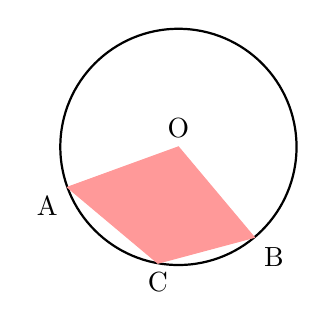
\begin{tikzpicture}
    \draw [thick](0,0) circle(1.5cm);
    \filldraw [red!40] (0,0)--(200:1.5cm)--(260:1.5cm)--(310:1.5cm)--cycle;
   \node [above] (0,0) {O};
   \node [below left] at (200:1.5cm) {A};
   \node [below] at (260:1.5cm) {C};
   \node [below right] at (310:1.5cm) {B};
\end{tikzpicture}
\begin{asy}
    size(200,0);
    draw((0,3)--(2,3),Arrow);
    draw((0,2)--(2,2),EndArrow);
    draw((0,1)--(2,1),BeginArrow);
    draw((0,0)--(2,0),Arrows);
    draw((0,-1)--(2,-1),MidArrow);
\end{asy}

\chapter{行程问题之巧用比例}
\section{知识点}
行程问题常和比例结合起来,题目虽然简洁,但是综合性强,而且形式多变,
运用比例知识解决复杂的行程问题经常考,而且要考都不简单。\par
我们知道行程问题里有三个量:速度、时间、距离,知道其中两个量就可以求
出第三个量。速度$\times$时间=距离;距离$\div$速度=时间;距离$\div$时间=速度。如果要用比例
做行程问题,这三个量之间的关系是:\par
\begin{enumerate}
\item 时间相同,速度比=距离比;
\item  速度相同,时间比=距离比;
\item  距离相同,速度比=时间的反比。
\end{enumerate}
\section{典型例题}
\begin{example}
    客车和货车同时从甲、乙两城之间的中点向相反的方向行驶, 3 小时后,客车
到达甲城,货车离乙城还有30 千米.已知货车的速度是客车的3/4,甲、乙两城相
距多少千米?
\end{example}
\vspace{2.5cm}
\begin{example}
    甲、乙两车同时从A、B 两地相向而行,它们相遇时距A 、B 两地中心处8
千米,已知甲车速度是乙车的1.2 倍,求A、B 两地的距离。
\end{example}
\vspace{2.5cm}
\begin{example}
    甲、乙两车分别从A 、B 两地同时出发,相向而行,甲车每小时行48 千米,
乙车每小时行42 千米。当乙车行至全程的$\frac{7}{20}$时,甲车距中点还有24 千米, A 、B
两地相距多少千米?
\end{example}
\vspace{2.5cm}
\begin{example}
    甲、乙两辆汽车同时从A、B 两地相向而行,甲行到全程的$\frac{3}{7}$的地方与乙相遇。
甲每小时行30 千米,乙行完全程需7 小时。求A、B 两地之间的路程。
\end{example}
\vspace{2.5cm}
\begin{example}
    一列货车和一列客车同时从甲乙两地相向开出, 已知客车的速度是货车的速度的
$\frac{2}{3}$,两车相遇时,客车比货车少行8 千米。求甲、乙两地间的距离。
\end{example}
\vspace{2.5cm}
\begin{example}
    甲、乙两车分别从A 、B 两地同时出发,相向而行,甲车每小时行56 千米,乙
车每小时行40 千米。当乙车行至全程的$\frac{2}{5}$时,甲车已超过中点12 千米, A 、B 两
地相距多少千米?
\end{example}
\vspace{2.5cm}
\begin{example}
    甲、乙两人分别从A、B 两地相向而行,甲行了全程的$\frac{5}{11}$ ,正好与乙相遇,已
    知甲每小时行4.5 千米,乙行完全程要5.5 小时,求A、B 两地相距多少千米?
\end{example}
\vspace{2.5cm}
\begin{example}
    客车和货车同时从A、B 两地相对开出, 货车的速度是客车的$\frac{2}{3}$ 。两车在离两地
中点30 千米处相遇。A、B 两地相距多少千米?
\end{example}
\vspace{2.5cm}
\begin{example}
    甲、乙两车分别从A、B 两地同时出发,相向而行,甲车速度是乙车速度的
$\frac{5}{6}$当乙车行至全程的$\frac{2}{5}$时,甲车距中点还有30 千米, A、B 两地相距多少千米?
\end{example}
\vspace{2.5cm}
\chapter{图示法解分数应用题}
\section{知识点}
图示法就是用线段图(或其它图形)把题目中的已知条件和问题表示出来,这
样可以把抽象的数量关系具体化,往往可以从图中找到解题的突破口。运用图示法
教学应用题,是培养思维能力的有效方法之一。\par
图示法不仅可以形象地、直观地反映分数应用题中的“对应量和对应分率”间
的关系,启发学生的解题思路,帮助学生找到解题的途径,而且通过画图的训练,
可以调动学生思维的积极性,提高学生分析问题和解决问题的能力。
\section{典型例题}
\begin{example}
    一条鱼重的$\frac{3}{5}$加上$\frac{3}{4}$千克就是这条鱼的重量,这条鱼重多少千克?
\end{example}
\vspace{2.5cm}
\begin{example}
    一桶油第一次用去$\frac{1}{5}$,第二次比第一次多用去20 千克,还剩下22 千克。原
来这桶油有多少千克?
\end{example}
\vspace{2.5cm}
\begin{example}
    缝纫机厂女职工占全厂职工人数的$\frac{7}{20}$,比男职工少144 人,缝纫机厂共有职
工多少人?
\end{example}
\vspace{2.5cm}
\begin{example}
    张亮从甲城到乙城,第一天行了全程的40\%,第二天行了全程的$\frac{9}{20}$,距乙城还
    有18 千米,甲、乙两城相距多少千米?
\end{example}
\vspace{2.5cm}
\begin{example}
    李玲看一本书,第一天看了全书的$\frac{1}{6}$,第二天看了18 页,这时正好看了全书的
一半。李玲第一天看书多少页?
\end{example}
\vspace{2.5cm}
\begin{example}
    某工程队修筑一条公路,第一周修了这段公路的$\frac{1}{4}$,第二周修了这段公路的
$\frac{2}{7}$。第二周比第一周多修了2 千米,这段公路全长多少千米?
\end{example}
\vspace{2.5cm}
\begin{example}
    汽车从学校出发到太湖玩,$\frac{6}{7}$小时行驶了全程的$\frac{3}{4}$
,这时距太湖边还有4 千米。
照这样的速度,行完全程共用多少小时?
\end{example}
\vspace{2.5cm}
\begin{example}
    某书店运来一批连环画。第一天卖出1800 本,第二天卖出的本数比第一天多
$\frac{1}{9}$,余下总数的$\frac{3}{7}$ 正好第三天全部卖完,这批连环画共有多少本?
\end{example}
\vspace{2.5cm}
\begin{example}
    一辆汽车从甲地开往乙地,第1 小时行了$\frac{1}{7}$,第2 小时比第1 小时少行了16 千
米,这时汽车距甲地94 千米。甲、乙两地相距多少千米?
\end{example}
\vspace{2.5cm}
\begin{example}
    水果店购进一批水果,第一天卖了30\%,第二天卖出余下的50\%,这两天共
卖出195 千克。这批水果共多少千克?
\end{example}
\vspace{2.5cm}
\begin{example}
    用绳子测井深,把绳子折成三股来量,井外余$\frac{4}{3}$米,把绳子折成四股来量,
井外余$\frac{1}{3}$米,井深多少米?
\end{example}
\vspace{2.5cm}

\chapter{二次根式}
\section{二次根式的概念及有意义的条件}
\subsection{概念}
一般地,我们把形如$\sqrt{a}(a\geq 0)$的式子叫做二次根式. $"\sqrt{~~}"$称为二次根号.
$$
\text{两个必备特征} \begin{cases}  
\text{外貌特征:含有$\sqrt{~~}$}\\
\text{内在特征:被开方数$a\geq 0$}
\end{cases}
$$
\subsection{有意义的条件}
\begin{enumerate}
    \item 单个二次根式如$\sqrt{A}$有意义的条件:$A\geq 0$;
    \item 多个二次根式相加如 $\sqrt{A}+\sqrt{B}+\ldots+\sqrt{N}$                         有意义的
    $A \geqslant 0,B \geqslant 0 ,\ldots N \geqslant 0$
    \item 二次根式作为分式的分母如$\frac{B}{\sqrt{A}}$有意义的条件: 
    $A>0$;
    \item 二次根式与分式的和如$\sqrt{A}+\frac{1}{B}$有意义的条件:
    $A \geq 0\text{且} B\neq 0$.


\end{enumerate}
\subsection{例题分析}
\begin{example}下列各式中,哪些是二次根式?哪些不是?\par
(1).$\sqrt{32}$ \hfil (2).6 \hfil (3).$\sqrt{-12}$ \hfil (4).$\sqrt{-m}(\leqslant 0)$\par
(5).$\sqrt{xy}(\text{x,y异号})$  \hfil (6).$\sqrt{a^2+1}$\hfil (7).$\sqrt[3]{5}$
\end{example}
\begin{example}
    当x是怎样的实数时,下列在实数范围内有意义?\par
    (1).$\sqrt{x-2}$\hfil (2).$\dfrac{1}{\sqrt{x-1}}$\hfil (3).$\dfrac{\sqrt{x+3}}{x-1}$\par
    \vspace{2cm}
    (4).$\sqrt{-x^{2}+2 x-1}$ \hfil  (5).$\sqrt{-x^{2}-2 x-3}$
\end{example}
\vspace{2cm}
\subsection{习题}
\begin{enumerate}
    \item  下列各式:$\sqrt{3}, \sqrt{-5},\sqrt{a^{2}} ,\sqrt{x-1}(x \geqslant 1) , \sqrt[3]{27} ,\sqrt{x^{2}+2 x+1}$
    一定是二次根式的个数有 (\qquad)
    \begin{tasks}(4)
        \task 3个
        \task 3个
        \task 5个
        \task 6个
    \end{tasks} \
    \item 若式子$\sqrt{\dfrac{x-1}{2}}$在实数范围内有意义,则x的取值 
    范围是    
    \item   若式子$\dfrac{1}{x-2}+\sqrt{x}$在实数范围内有意义,则x的  
    取值范围是 
    \end{enumerate}
    \section{二次根式的性质}
    二次根式的实质是表示一个非负数(或式)的算术平方根.对于任意一个二次根式$\sqrt{a}$ ,我们知道:
    \begin{enumerate}
       \item a为被开方数,为保证其有意义,可知$a \geq 0$;
       \item $\sqrt{a}$表示一个数或式的算术平方根,可知$\sqrt{a} \geq 0$.
       \item $(\sqrt{a})^{2}=a(a \geqslant 0)$
       \item $\sqrt{a^{2}}=|a|=\left\{\begin{array}{ll}{a} & {(a \geqslant 0)} \\ {-a} & {(a<0)}\end{array}\right.$
   \end{enumerate}
   \subsection{例题分析}
      \begin{example}   
            计算:\par
            (1).$(\sqrt{\dfrac{4}{7}})^2$   \hfil (2).$(4\sqrt{3})^2$\par 
            \vspace{2cm}
            (3). $\sqrt{(-5)^2}$ \hfil  (4).$-\sqrt{(-\dfrac{1}{7})^2}$ 
            \vspace{2cm}  
      \end{example} 
      \begin{example}
          实数$a,b$在数轴上对应的点位置如图所示,化简$|a|+\sqrt{(a-b)^2}$结果为\par
       
             
         \begin{figure}[h]
            \centering
             
       
          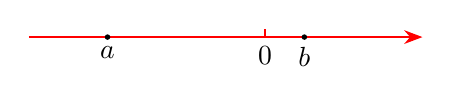
\begin{tikzpicture}
          \draw [-Stealth,thick,red](-3cm,0)--(-1cm,0)--(2cm,0);
          \node (0,0) [below]{0};
          \node [below] at (-2cm,0)  {$a$};
          \node [below] at (0.5cm,0) {$b$};
          \fill (-2cm,0) circle (1pt);
          \fill (0.5cm,0) circle (1pt);
          \draw [red,thick](0,0)--(0,3pt);
        
          \end{tikzpicture}
          \caption{\label{fig: } }
        \end{figure}
      \end{example}
      
            \begin{example}
        若$|a-2|+\sqrt{b-3}+(c-4)^{2}=0$,求$a-b+c$的值.
      \end{example}
      \vspace{2cm}
      
      \begin{example}
        已知$y=\sqrt{x-3}+\sqrt{3-x}+8$,求$3 x+2 y$的算术平方根.
      \end{example}
      \vspace{2cm}
      \begin{example}
        已知a,b为等腰三角形的两条边长,且a,b满足$b=\sqrt{3-a}+\sqrt{2 a-6}+4$,求此三角形的周长
      \end{example}
      \vspace{1.7cm}
      \subsection{练习}
      \begin{enumerate}
       \item  已知$|3 x-y-1|$和$\sqrt{2 x+y-4}$互为相反数,求$x+4 y$的平方根.
       \item \vspace{1.7cm} 下列式子中,不属于二次根式的是
       \begin{tasks}(4)
           \task $\sqrt{5}$
           \task $\sqrt{a^{2}}$
           \task $\sqrt{-7}$
           \task $\sqrt{\frac{1}{2}}$
        \end{tasks}
           \item  式子$\dfrac{-2}{\sqrt{3 x-6}}$有意义的条件是  
    \begin{tasks}(4B)
    \task $x>2$
    \task $x \geq 2$
    \task $x<2$
    \task $x \leqslant 2$
    \end{tasks}      
       
       \item 当a是怎样的实数时,下列各式在实数范围内有意义?   \par
       (1)$\sqrt{a-1}$ \hfil (2)$\sqrt{2 a+3}$ \hfil (3)$\sqrt{-a}$ \hfil (4)$\sqrt{\dfrac{2}{5-a}}$
       \item  若二次根式$\dfrac{\sqrt{m-2}}{|m^{2}-m-2|}$有意义,求m的取值范围
        \item  \vspace{2cm}  无论x取任何实数,代数式$\sqrt{x^{2}+6 x+m}$都有意义,求m的取值范围.
        \item \vspace{2cm}  若x,y是实数,且$y<\sqrt{x-1}+\sqrt{1-x}+\frac{1}{2}$,求 $\dfrac{|1-y|}{y-1}$       的值
        \item \vspace{2cm}  当x为何值时,$\sqrt{x(x-1)}$有意义?
        \item \vspace{2cm}  当x为何值时,$\sqrt{\dfrac{x-2}{2 x+1}}$有意义?
    \end{enumerate}
      

                     




\chapter{按比例分配}
\section{知识点}
把一个总量按照一定的比分成若干个分量的应用题,叫做按比例分配。按比例
分配的方法是,将按已知比分配变为按份数分配,把比的各项相加得到总份数,各
项与总份数之比就是各个分量在总量中所占的分率,由此可求得各个分量。\par
解答按比例分配应用题的步骤是\par
第一:求出按比例分配的总数量;\par
第二:找出分配的比,并求各个部分占总数量的几分之几;\par 
第三:用总数量乘以部分量占总数的几分之几得到各部分量。
\section{例题分析}
\begin{example}
    用60 厘米长的铁丝围成一个三角形,三角形三条边的比是3∶4∶5。三条边
    的长各是多少厘米? 
\end{example}
\vspace{3cm}
\begin{example}
    学校把植树560 棵的任务按人数分配给五年级三个班,已知一班有47 人,二
班有48 人,三班有45 人,三个班各植树多少棵?
\end{example}
\vspace{3cm}
\begin{example}
    某工厂第一、二、三车间人数之比为8∶12∶ 21,第一车间比第二车间少80
人,三个车间共多少人?
\end{example}
\vspace{3cm}
\section{练习}
\vspace{-0.4cm}
\begin{exercise}
    建筑工人用水泥、沙子、石子按2: 3:5 配制成96 吨的混凝土,需要水泥、沙
    子、石子各多少吨?  
\end{exercise}
\vspace{3.2cm}
\begin{exercise}
    把280 棵树苗栽在两块长方形地上,一块长15 米,宽8 米;另一块长12 米,宽
4 米,如按面积大小分配栽种,这两块地分别要栽多少棵?
\end{exercise}
\vspace{3.2cm}
\begin{exercise}
    甲、乙两个建筑队原有水泥的重量比是4:3。当甲队给乙队54 吨水泥后,甲、
    乙两队的水泥的重量比是3:4。原来甲队有水泥多少吨?
\end{exercise}
\vspace{3.2cm}
\begin{exercise}
    某农场把61600 亩耕地进行规划,其中粮田与棉田的比是7: 2,棉田与其他作
物田的比是6:1,每种耕地各有多少亩?
\end{exercise}
\vspace{3.2cm}
\begin{exercise}
    王晓峰的书架有上、中、下三层。上层存书本数与存书总数的比是5:21。如果
从下层拿18 本书放到上层,则每层书架的存书本数相等。这个书架共有存书多少
本?
\end{exercise}
\vspace{3.2cm}
\begin{exercise}
    甲、乙两个工地上原来水泥袋数的比是2:1,甲地用去125 袋后,甲、乙两工
地水泥袋数的比为3:4,甲、乙两工地原有水泥多少袋?
\end{exercise}
\vspace{3.2cm}
\begin{exercise}
    纸箱里有红绿黄三色球,红色球的个数是绿色球的$\frac{3}{4}$ ,绿色球的个数与黄色
球个数的比是4: 5,已知绿色球与黄色球共81 个,问三色球各有多少个?
\end{exercise}
\vspace{3.2cm}
\begin{exercise}
    从前有个牧民,临死前留下遗言,要把17 只羊分给三个儿子,大儿子分总
数的$\frac{1}{2}$ ,二儿子分总数的$\frac{1}{3}$ ,三儿子分总数的
$\frac{1}{9}$,并规定不许把羊宰割分,求三个
儿子各分多少只羊?
\end{exercise}
\vspace{3.2cm}

\end{document}
